\chapter{Probabilitat}

\index{probabilitat}

Una \key{probabilitat} és un nombre real entre $0$ i $1$ que indica
quan probable és un esdeveniment.  Si un esdeveniment passarà segur,
la seva probabilitat és 1, i si un esdeveniment és impossible, la seva
probabilitat és 0. La probabilitat d'un esdeveniment s'indica
$P(\cdots)$ on els tres punts descriuen l'esdeveniment.

Per exemple, quan es llança un dau, el resultat és un nombre enter
entre $1$ i $6$, i la probabilitat de cada resultat és $1/6$. Per
exemple, podem calcular les probabilitats següents:


\begin{itemize}[noitemsep]
\item $P(\textrm{''el resultat és 4''})=1/6$
\item $P(\textrm{''el resultat no és 6''})=5/6$
\item $P(\textrm{''el resultat és parell''})=1/2$
\end{itemize}


\section{Càlcul}

Per a calcular la probabilitat d'un esdeveniment fem servir la
combinatòria o simulem el procés que genera l'esdeveniment. Per
exemple exemple, calculem la probabilitat de treure tres cartes amb el
mateix valor d'una baralla de cartes barrejades (per exemple,
$\spadesuit 8$, $\clubsuit 8$ i $\diamondsuit 8$).

\subsubsection*{Mètode 1}

Podem calcular la probabilitat mitjançant la fórmula


\[\frac{\textrm{nombre de resultats desitjats}}{\textrm{nombre total de resultats}}.\]


En aquest problema, els resultats desitjats són aquells en què el
valor de cada carta és el mateix. Hi ha $13 {4 \choose 3}$ resultas
d'aquesta mena, perquè hi ha $13$ possibilitats pel valor de les
cartes i ${4 \choose 3}$ maneres de triar $3$ colls (pals) entre
els $4$ colls possibles.

Hi ha un total de ${52 \choose 3}$ resultats, perquè triem 3 cartes
d'entre 52 cartes. Per tant, la probabilitat de l'esdeveniment és


\[\frac{13 {4 \choose 3}}{{52 \choose 3}} = \frac{1}{425}.\]


\subsubsection*{Mètode 2}

Una altra manera de calcular la probabilitat és simular el procés que
genera l'esdeveniment. En aquest exemple, treiem tres cartes, de
manera que el procés consta de tres passos. Exigim que cada pas del
procés tingui èxit.

El coll de la primera carta sempre té èxit, perquè no hi ha
restriccions. El segon pas té èxit amb una probabilitat de $3/51$,
perquè queden 51 cartes i 3 d'elles tenen el mateix valor que la
primera. De la mateixa manera, el tercer pas té èxit amb una
probabilitat de $2/50$.

La probabilitat que tot el procés tingui èxit és


\[1 \cdot \frac{3}{51} \cdot \frac{2}{50} = \frac{1}{425}.\]


\section{Esdeveniments}

Un esdeveniment en teoria de probabilitats es pot representar com un
conjunt
\[A \subset X,\]
on $X$ conté tots els resultats possibles i $A$ és un subconjunt de
resultats. Per exemple, quan es llença un dau, els resultats són
\[X = \{1,2,3,4,5,6\}.\]
Per exemple, l'esdeveniment ''el resultat és parell'' es correspon
al conjunt
\[A = \{2,4,6\}.\]


A cada resultat $x$ li assignem una probabilitat $p(x)$. La
probabilitat $P(A)$ d'un esdeveniment $A$ es pot calcular com una
suma de probabilitats dels resultats mitjançant la fórmula
\[P(A) = \sum_{x \in A} p(x).\]
Per exemple, quan es llança un dau, $p(x)=1/6$ per a cada resultat
$x$, de manera que la probabilitat de l'esdeveniment ''el resultat
és parell'' és
\[p(2)+p(4)+p(6)=1/2.\]


La probabilitat total dels resultats en $X$ ha de ser 1, és a dir,
$P(X)=1$.

Com que els esdeveniments de la teoria de la probabilitat són
conjunts, podem manipular-los mitjançant operacions de conjunts
estàndard:


\begin{itemize}
\item El \key{complement} $\bar A$ significa
''$A$ no passa''.
Per exemple, quan es llança un dau,
el complement de $A=\{2,4,6\}$ és
$\bar A = \{1,3,5\}$.
\item La \key{union} $A \cup B$ significa
''$A$ o $B$ passa''.
Per exemple, la unió de
$A=\{2,5\}$
i $B=\{4,5,6\}$ és
$A \cup B = \{2,4,5,6\}$.
\item La \key{intersecció} $A \cap B$ significa
''$A$ i $B$ passen''.
Per exemple, la intersecció de
$A=\{2,5\}$ i $B=\{4,5,6\}$ és
$A \cap B = \{5\}$.
\end{itemize}



\subsubsection{Complement}

La probabilitat del complement $\bar A$ es calcula mitjançant la
fórmula
\[P(\bar A)=1-P(A).\]


De vegades, podem resoldre un problema fàcilment amb
complements resolent el problema contrari. Per exemple, la
probabilitat d'obtenir almenys un sis en llançar un dau deu vegades és
\[1-(5/6)^{10}.\]


Aquí $5/6$ és la probabilitat que el resultat d'un sol llançament no
sigui sis, i $(5/6)^{10}$ és la probabilitat que cap dels deu
llançaments sigui un sis. El complement d'això és la resposta al
problema.

\subsubsection{Unió}

La probabilitat de la unió $A \cup B$ es calcula mitjançant la fórmula
\[P(A \cup B)=P(A)+P(B)-P(A \cap B).\]
Per exemple, quan es llança un dau, la unió dels esdeveniments
\[A=\textrm{''el resultat és parell''}\]
i
\[B=\textrm{''el resultat és inferior a 4''}\]
és
\[A \cup B=\textrm{''el resultat és parell o inferior a 4''},\]
i la seva probabilitat és
\[P(A \cup B) = P(A)+P(B)-P(A \cap B)=1/2+1/2-1/6=5/6.\]

Si els esdeveniments $A$ i $B$ són \key{disjunts}, és a dir, $A \cap
B$ està buit, la probabilitat de l'esdeveniment $A \cup B$ és
simplement


\[P(A \cup B)=P(A)+P(B).\]


\subsubsection{Probabilitat condicionada}

\index{probabilitat condicionada}

La \key{probabilitat condicionada}
\[P(A | B) = \frac{P(A \cap B)}{P(B)}\]
és la probabilitat que passi $A$ assumint que passa $B$. Per tant,
quan es calcula la probabilitat de $A$, només considerem els resultats
que també pertanyen a $B$.

Utilitzant els conjunts anteriors,
\[P(A | B)= 1/3,\]
perquè els resultats de $B$ són $\{1,2,3\}$, i un d'ells és
parell. Aquesta és la probabilitat d'un resultat parell si sabem que
el resultat està entre $1 \ldots 3$.

\subsubsection{Intersecció}

\index{independència}

Utilitzant la probabilitat condicionada, la probabilitat de la
intersecció $A \cap B$ es pot calcular mitjançant la fórmula
\[P(A \cap B)=P(A)P(B|A).\]
Els esdeveniments $A$ i $B$ són \key{independents} si
\[P(A|B)=P(A) \hspace{10px}\textrm{and}\hspace{10px} P(B|A)=P(B),\]
el que significa que el fet que passi $B$ no modifica la probabilitat
de $A$, i viceversa. En aquest cas, la probabilitat de la intersecció
és
\[P(A \cap B)=P(A)P(B).\]
Per exemple, en treure una carta d'una baralla, els esdeveniments
\[A = \textrm{''el coll és piques''}\]
i
\[B = \textrm{''el valor és quatre''}\]
són independents. Per tant, l'esdeveniment
\[A \cap B = \textrm{''la carta és el quatre de piques''}\]
passa amb probabilitat
\[P(A \cap B)=P(A)P(B)=1/4 \cdot 1/13 = 1/52.\]

\section{Variables aleatòries}

\index{variable aleatòria}

Una \key{variable aleatòria} és un valor generat per un procés
aleatori. Per exemple, quan es llancen dos daus, una possible variable
aleatòria és
\[X=\textrm{''the sum of the outcomes''}.\]
Per exemple, si els resultats són $[4,6]$ (és a dir, primer tirem un
quatre i després un sis), aleshores el valor de $X$ és 10.

Denotem $P(X=x)$ la probabilitat que el valor d'una variable aleatòria
$X$ sigui $x$\footnote{(N. del T.) Les variables aleatòries ens
permeten representar esdeveniments (conjunts de resultats) de manera
compacta. En aquest cas, $P(X=x)$ és una manera d'abreujar $P(\{r |
X(r)=x\})$, és a dir, la probabilitat de l'esdeveniment format per
tots aquells resultats $r$ que tenen valor assignat $X(r)$ igual a una
constant $x$.}. Per exemple, en llançar dos daus, $P(X=10)=3/36$,
perquè el nombre total de resultats és 36 i hi ha tres maneres
possibles d'obtenir la suma 10: $[4,6]$, $[5,5]$ i $[6,4]$.

\subsubsection{Valor esperat}

\index{valor esperat}

La \key{valor esperat} $E[X]$ indica el valor mitjà d'una variable
aleatòria $X$. El valor esperat es pot calcular com la suma
\[\sum_x P(X=x)x,\]
on $x$ itera per tots els valors possibles de $X$.

Per exemple, quan es llança un dau, el resultat esperat és
\[1/6 \cdot 1 + 1/6 \cdot 2 + 1/6 \cdot 3 + 1/6 \cdot 4 + 1/6 \cdot 5 + 1/6 \cdot 6 = 7/2.\]


Una propietat útil dels valors esperats és que són \key{lineals}. Això
vol dir que la suma $E[X_1+X_2+\cdots+X_n]$ sempre és igual a la suma
$E[X_1]+E[X_2]+\cdots+E[X_n]$. Aquesta fórmula és certa encara que les
variables aleatòries depenguin les unes de les altres.

Per exemple, quan es llança dos daus, la suma esperada és
\[E[X_1+X_2]=E[X_1]+E[X_2]=7/2+7/2=7.\]


Considerem ara un problema en què $n$ boles es col·loquen
aleatòriament en $n$ caixes, i la nostra tasca és calcular el nombre
esperat de caixes buides. Cada bola té la mateixa probabilitat de ser
col·locada en qualsevol de les caixes. Per exemple, si $n=2$, les
probabilitats són les següents:
\begin{center}
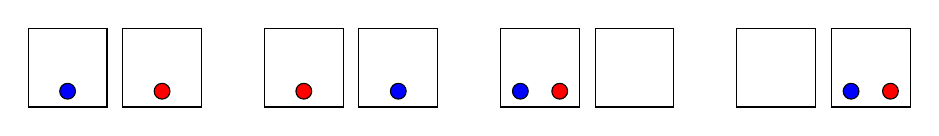
\begin{tikzpicture}
\draw (0,0) rectangle (1,1);
\draw (1.2,0) rectangle (2.2,1);
\draw (3,0) rectangle (4,1);
\draw (4.2,0) rectangle (5.2,1);
\draw (6,0) rectangle (7,1);
\draw (7.2,0) rectangle (8.2,1);
\draw (9,0) rectangle (10,1);
\draw (10.2,0) rectangle (11.2,1);

\draw[fill=blue] (0.5,0.2) circle (0.1);
\draw[fill=red] (1.7,0.2) circle (0.1);
\draw[fill=red] (3.5,0.2) circle (0.1);
\draw[fill=blue] (4.7,0.2) circle (0.1);
\draw[fill=blue] (6.25,0.2) circle (0.1);
\draw[fill=red] (6.75,0.2) circle (0.1);
\draw[fill=blue] (10.45,0.2) circle (0.1);
\draw[fill=red] (10.95,0.2) circle (0.1);
\end{tikzpicture}
\end{center}
En aquest cas, el nombre esperat de caixes buides és
\[\frac{0+0+1+1}{4} = \frac{1}{2}.\]
En el cas general, la probabilitat que una sola caixa estigui buida és
\[\Big(\frac{n-1}{n}\Big)^n,\]
perquè no hem de posar cap bola. Per tant, utilitzant la linealitat,
el nombre esperat de caixes buides és
\[n \cdot \Big(\frac{n-1}{n}\Big)^n.\]


\subsubsection{Distribucions}

\index{distribució}

La \key{distribució} d'una variable aleatòria $X$ indica la
probabilitat de tots els valors que $X$ pot tenir. La distribució
consta de valors $P(X=x)$. Per exemple, quan es llança dos daus, la
distribució de la seva suma és:
\begin{center}
\small {
\begin{tabular}{r|rrrrrrrrrrrrr}
$x$ & 2 & 3 & 4 & 5 & 6 & 7 & 8 & 9 & 10 & 11 & 12 \\
$P(X=x)$ & $1/36$ & $2/36$ & $3/36$ & $4/36$ & $5/36$ & $6/36$ & $5/36$ & $4/36$ & $3/36$ & $2/36$ & $1/36$ \\
\end{tabular}
}
\end{center}


\index{distribució uniforme} En una \key{distribució uniforme}, la
variable aleatòria $X$ té $n$ valors possibles $a,a+1,\ldots,b$ i la
probabilitat de cada valor és $1/n$ . Per exemple, quan es llança un
dau, $a=1$, $b=6$ i $P(X=x)=1/6$ per a cada valor $x$.

El valor esperat de $X$ en una distribució uniforme és
\[E[X] = \frac{a+b}{2}.\]


\index{distribució binomial} En una \key{distribució binomial}, es fan
$n$ intents i la probabilitat que un sol intent tingui èxit és $p$. La
variable aleatòria $X$ compta el nombre d'intents amb èxit i la
probabilitat d'un valor $x$ és
\[P(X=x)=p^x (1-p)^{n-x} {n \choose x},\]
on $p^x$ i $(1-p)^{n-x}$ es corresponen amb els intents exitosos i
infructuosos, i ${n \choose x}$ és el nombre de maneres de triar
l'ordre dels intents.

Per exemple, quan es llança un dau deu vegades, la probabilitat de
treure un sis exactament tres vegades és $(1/6)^3 (5/6)^7 {10 \choose
  3}$.

El valor esperat de $X$ en una distribució binomial és
\[E[X] = pn.\]


\index{distribució geomètrica} En una \key{distribució geomètrica}, la
probabilitat que un intent tingui èxit és $p$, i continuem fins que es
produeix el primer èxit. La variable aleatòria $X$ compta el nombre
d'intents necessaris i la probabilitat d'un valor $x$ és [[[[40]]]] on
$(1-p)^{x-1}$ es correpon amb els intents infructuosos i $p$ es
correspon al primer intent amb èxit.

Per exemple, si llancem un dau fins que treiem un sis, la probabilitat
que el nombre de llançaments sigui exactament 4 és $(5/6)^3 1/6$.

El valor esperat de $X$ en una distribució geomètrica és
\[E[X]=\frac{1}{p}.\]


\section{Cadenes de Markov}

\index{Cadena de Markov}

Una \key{cadena de Markov} % \footnote{A. A. Markov (1856--1922) % va ser un matemàtic rus.}
és un procés aleatori que consta d'estats i transicions entre
ells. Per a cada estat coneixem les probabilitats de passar als
altres estats. Una cadena de Markov es pot representar com un graf els
nodes del qual són estats i les arestes són transicions.

Per exemple, considereu el problema on estem a la planta 1 d'un
edifici de $n$ plantes. A cada pas, caminem aleatòriament un pis cap
amunt o un pis cap avall, excepte si estem al primer o últim pis, on
sempre caminem cap amunt o cap avall respectivament. Quina és la
probabilitat d'estar al pis $m$ després de $k$ passos?

En aquest problema, cada pis de l'edifici es correspon a un estat en
una cadena de Markov. Per exemple, si $n=5$, el graf és el següent:


\begin{center}
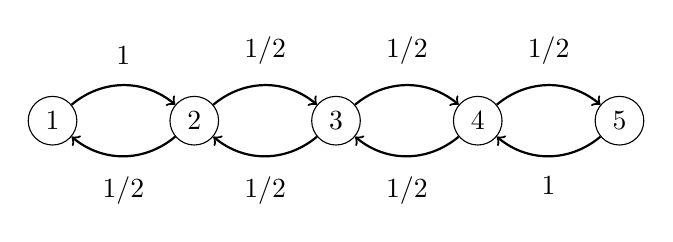
\begin{tikzpicture}[scale=0.9]
\node[draw, circle] (1) at (0,0) {$1$};
\node[draw, circle] (2) at (2,0) {$2$};
\node[draw, circle] (3) at (4,0) {$3$};
\node[draw, circle] (4) at (6,0) {$4$};
\node[draw, circle] (5) at (8,0) {$5$};

\path[draw,thick,->] (1) edge [bend left=40] node[font=\small,label=$1$] {} (2);
\path[draw,thick,->] (2) edge [bend left=40] node[font=\small,label=$1/2$] {} (3);
\path[draw,thick,->] (3) edge [bend left=40] node[font=\small,label=$1/2$] {} (4);
\path[draw,thick,->] (4) edge [bend left=40] node[font=\small,label=$1/2$] {} (5);

\path[draw,thick,->] (5) edge [bend left=40] node[font=\small,label=below:$1$] {} (4);
\path[draw,thick,->] (4) edge [bend left=40] node[font=\small,label=below:$1/2$] {} (3);
\path[draw,thick,->] (3) edge [bend left=40] node[font=\small,label=below:$1/2$] {} (2);
\path[draw,thick,->] (2) edge [bend left=40] node[font=\small,label=below:$1/2$] {} (1);

%\path[draw,thick,->] (1) edge [bend left=40] node[font=\small,label=below:$1$] {} (2);
\end{tikzpicture}
\end{center}


La distribució de probabilitat d'una cadena de Markov és un vector
$[p_1,p_2,\ldots,p_n]$, on $p_k$ és la probabilitat que l'estat actual
sigui $k$. La fórmula $p_1+p_2+\cdots+p_n=1$ sempre és vàlida.

En l'escenari anterior, la distribució inicial és $[1,0,0,0,0]$,
perquè sempre comencem al pis 1. La següent distribució és
$[0,1,0,0,0]$, perquè només podem passar del pis 1 al pis 2. Després
d'això, podem moure un pis cap amunt o un pis cap avall, de manera que
la següent distribució és $[1/2,0,1/2,0,0]$ i així successivament.

Una manera eficient de simular recorreguts en cadenes de Markov és amb
la programació dinàmica. La idea és guardar-nos la distribució de
probabilitat i, a cada pas, iterar per totes les possibles maneres de
moure's des de cada estat. Amb aquest mètode podem simular un recorregut
de $m$ passos en temps $O(n^2 m)$.

Les transicions d'una cadena de Markov també es poden representar com
una matriu que actualitza la distribució de probabilitat. En
l'escenari anterior, la matriu és

\[ \begin{bmatrix} 0 & 1/2 & 0 & 0 & 0 \\ 1 & 0 & 1/2 & 0 & 0 \\ 0 & 1/2 & 0 & 1/2 & 0 \\ 0 & 0 & 1/2 & 0 & 1 \\ 0 & 0 & 0 & 1/2 & 0 \\ \end{bmatrix}. \]

Quan multipliquem una distribució de probabilitat per aquesta matriu,
obtenim la nova distribució després de moure'ns un pas. Per exemple,
passem de la distribució $[1,0,0,0,0]$ a la distribució $[0,1,0,0,0]$
de la manera següent:

\[   \begin{bmatrix}   0 & 1/2 & 0 & 0 & 0 \\   1 & 0 & 1/2 & 0 & 0 \\   0 & 1/2 & 0 & 1/2 & 0 \\   0 & 0 & 1/2 & 0 & 1 \\   0 & 0 & 0 & 1/2 & 0 \\  \end{bmatrix}  \begin{bmatrix}   1 \\   0 \\   0 \\   0 \\   0 \\  \end{bmatrix} =  \begin{bmatrix}   0 \\   1 \\   0 \\   0 \\   0 \\  \end{bmatrix}. \]

Si calculem les potències de la matriu de manera eficient, podem
calcular la distribució després de $m$ passos en temps $O(n^3 \log
m)$.

\section{Algorismes aleatoris}

\index{algorisme aleatoris}

De vegades podem fer servir l'atzar per resoldre un problema, encara
que el problema no estigui relacionat amb probabilitats. Un
\key{algorisme aleatori} (\emph{randomized algorithm}) és un algorisme
que pren decisions aleatòries durant la seva execució.

\index{Algorisme de Monte Carlo}

Un \key{algorisme de Monte Carlo} és un algorisme aleatori que de
vegades pot donar una resposta incorrecta. Aquests algorismes són
útils quan la probabilitat de donar una resposta incorrecta és petita.

\index{Algorisme de Las Vegas}

Un \key{algorisme de Las Vegas} és un algorisme aleatori que sempre
dóna la resposta correcta, però que el seu temps d'execució varia
aleatòriament. L'objectiu és dissenyar un algorisme que sigui eficient
amb alta probabilitat.

A continuació, mostrem tres exemples de problemes que es poden
resoldre fent servir l'atzar.

\subsubsection{Estadístiques d'ordre}

\index{estadístiques d'ordre}

La $k$-èssima \key{estadistica d'ordre} d'un vector és l'element que
resulta a la posició $k$ després d'ordenar el vector en ordre
creixent. És fàcil calcular les estadístiques d'ordre en temps $O(n
\log n)$ ordenant primer el vector, però és realment necessari ordenar
tot el vector per a trobar un sol element?

Resulta que podem trobar l'estadística d'ordre amb un algorisme
aleatori sense ordenar el vector. L'algorisme, anomenat
\key{quickselect}\footnote{L'any 1961, CAR Hoare va publicar dos
algorismes eficients en mitjana: \index{quicksort} \index{quickselect}
\key{quicksort} \cite{hoa61a} per ordenar vectors i \key{quickselect}
\cite{hoa61b} per trobar estadístiques d'ordre.}, és un algorisme de
Las Vegas: el seu temps d'execució sol ser $O(n)$ però és $O(n^2)$ en
el pitjor dels casos.

L'algorisme tria un element aleatori $x$ del vector i mou els elements
més petits que $x$ a la part esquerra del vector i tots els altres
elements a la part dreta. Això triga temps $O(n)$ quan hi ha $n$
elements. Suposem que la part esquerra conté $a$ elements i la part
dreta conté $b$ elements. Si $a=k$, l'element $x$ és la $k$-èssima
l'estadística d'ordre. En cas contrari, si $a>k$, trobem recursivament
l'estadística d'ordre $k$-èssima a la part esquerra, i si $a<k$,
trobem recursivament l'estadística d'ordre $r$-èssima per a la part
dreta, on $r=ka$. La recerca continua de manera similar, fins que s'ha
trobat l'element.

Quan cada element $x$ es tria aleatòriament, la mida del vector es
redueix aproximadament a la meitat a cada pas, de manera que la
complexitat temporal de trobar la $k$-èssima estadística d'ordre és
d'aproximadament
\[n+n/2+n/4+n/8+\cdots < 2n = O(n).\]


El pitjor cas es quan l'algorisme requereix $O(n^2)$ temps, perquè és
possible que $x$ sempre es trii de manera que sigui un dels elements
més petits o més grans del vector, i siguin necessaris $O(n)$
passos. Tanmateix, la probabilitat que passi això és tan petita que
mai passa a la pràctica.

\subsubsection{Verificar multiplicacions de matrius}

\index{multiplicació de matrius}

El nostre següent problema és \emph{verificar} si passa $AB=C$ on $A$,
$B$ i $C$ són matrius de mida $n \times n$. Per descomptat, podem
resoldre el problema calculant de nou el producte $AB$ (en temps
$O(n^3)$ amb l'algorisme bàsic), però es podria esperar que verificar
la resposta hauria de ser més fàcil que calcular-la des de zero.

Resulta que podem resoldre el problema amb un algorisme de
Monte Carlo\footnote{R. M. Freivalds va publicar aquest algorisme
  l'any 1977 \cite{fre77}, i de vegades s'anomena \index{Algorisme de
    Freivalds} \key{Algorisme de Freivalds}.}, la complexitat temporal
del qual només és $O(n^2)$. La idea és senzilla: triem un vector
aleatori $X$ de $n$ elements, i calculem els vectors $ABX$ i $CX$. Si
$ABX=CX$, informem que $AB=C$, i en cas contrari informem que $AB \neq
C$.

La complexitat temporal de l'algorisme és $O(n^2)$, perquè podem
calcular els matrius $ABX$ i $CX$ en el temps $O(n^2)$. Podem calcular
el vector $ABX$ de manera eficient fent servir la representació
$A(BX)$, de manera que només calen dues multiplicacions de matrius de
mida $n \times n$ i $n \times 1$.

L'inconvenient de l'algorisme és que hi ha una petita possibilitat que
l'algorisme cometi un error quan troba que $AB=C$. Per exemple,
\[
 \begin{bmatrix}
  6 & 8 \\
  1 & 3 \\
 \end{bmatrix}
\neq
 \begin{bmatrix}
  8 & 7 \\
  3 & 2 \\
 \end{bmatrix},
\]
però
\[
 \begin{bmatrix}
  6 & 8 \\
  1 & 3 \\
 \end{bmatrix}
 \begin{bmatrix}
  3 \\
  6 \\
 \end{bmatrix}
=
 \begin{bmatrix}
  8 & 7 \\
  3 & 2 \\
 \end{bmatrix}
 \begin{bmatrix}
  3 \\
  6 \\
 \end{bmatrix}.
\]
A la pràctica, però, la probabilitat que l'algorisme cometi un error
és molt petita, i podem fer que encara sigui més petita verificant el
resultat per a diversos vectors aleatoris $X$ abans d'informar que
$AB=C$.

\subsubsection{Acolorir un graf}

\index{acolorir}

Donat un graf amb $n$ nodes i $m$ arestes, la nostra tasca és acolorir
els nodes del graf amb dos colors de manera que com a mínim $m/2$
arestes tinguin extrems amb colors diferents. Per exemple, al graf
\begin{center}
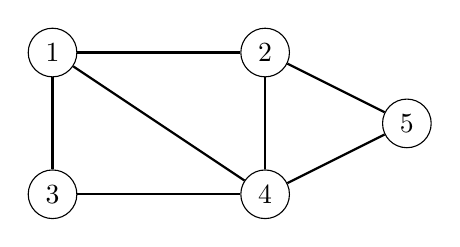
\begin{tikzpicture}[scale=0.9]
\node[draw, circle] (1) at (1,3) {$1$};
\node[draw, circle] (2) at (4,3) {$2$};
\node[draw, circle] (3) at (1,1) {$3$};
\node[draw, circle] (4) at (4,1) {$4$};
\node[draw, circle] (5) at (6,2) {$5$};

\path[draw,thick,-] (1) -- (2);
\path[draw,thick,-] (1) -- (3);
\path[draw,thick,-] (1) -- (4);
\path[draw,thick,-] (3) -- (4);
\path[draw,thick,-] (2) -- (4);
\path[draw,thick,-] (2) -- (5);
\path[draw,thick,-] (4) -- (5);
\end{tikzpicture}
\end{center}
una coloració vàlida és la següent:
\begin{center}
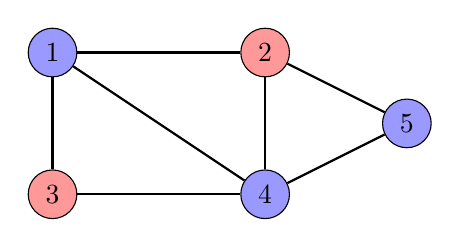
\begin{tikzpicture}[scale=0.9]
\node[draw, circle, fill=blue!40] (1) at (1,3) {$1$};
\node[draw, circle, fill=red!40] (2) at (4,3) {$2$};
\node[draw, circle, fill=red!40] (3) at (1,1) {$3$};
\node[draw, circle, fill=blue!40] (4) at (4,1) {$4$};
\node[draw, circle, fill=blue!40] (5) at (6,2) {$5$};

\path[draw,thick,-] (1) -- (2);
\path[draw,thick,-] (1) -- (3);
\path[draw,thick,-] (1) -- (4);
\path[draw,thick,-] (3) -- (4);
\path[draw,thick,-] (2) -- (4);
\path[draw,thick,-] (2) -- (5);
\path[draw,thick,-] (4) -- (5);
\end{tikzpicture}
\end{center}
El graf anterior conté 7 arestes i 5 d'elles tenen extrems amb colors
diferents, de manera que l'acoloració és vàlida.

El problema es pot resoldre amb un algorisme de Las Vegas que genera
coloracions aleatòries fins que troba una coloració vàlid. En una
coloració aleatòria, el color de cada node s'escull independentment
amb probabilitat $1/2$ per a cada color.

En una coloració aleatòria, la probabilitat que els dos extrems d'una
aresta tinguin colors diferents és $1/2$. Per tant, el nombre esperat
d'arestes amb colors diferents als extrems és $m/2$. Com que s'espera
que una coloració aleatòria sigui vàlida, ràpidament trobarem una
coloració vàlida a la pràctica.

